% NeuroCam manual - User guide subset - Top level
% Written by Christopher Thomas.
% Copyright (c) 2021 by Vanderbilt University. This work is released under
% the Creative Commons Attribution-ShareAlike 4.0 International License.

\documentclass[letterpaper,11pt]{report}
\usepackage[letterpaper]{geometry}
\usepackage{graphicx}
\usepackage{verbatim}

\geometry{nohead,footskip=0.3in,margin=0.75in}

% Force my paragraph style, darnit.
\usepackage{indentfirst}
\setlength{\parskip}{\baselineskip}

% Custom macros.
\newcommand{\fixme}[1]{\textbf{FIXME: #1}}

% Document body.
\begin{document}

% Title page.

\pagestyle{empty}

\begin{center}
%
\vspace*{1.5in}
{\Huge NeuroCam System User Guide} \\
{\footnotesize Written by Christopher Thomas -- \today.} \\
%
\vspace*{1in}
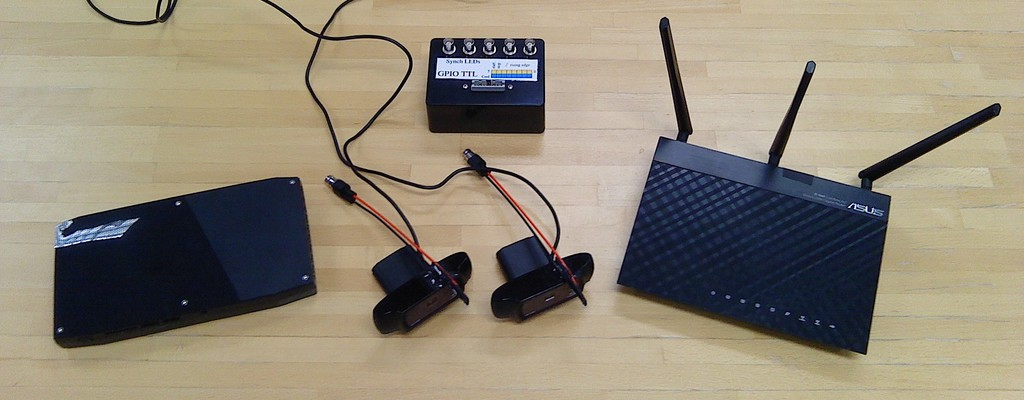
\includegraphics[width=0.9\textwidth]{pics-system/sys-all-d.jpg} \\
%
\vfill
{\footnotesize % NeuroCam manual - License tagline.
% Written by Christopher Thomas.
% Copyright (c) 2021 by Vanderbilt University. This work is released under
% the Creative Commons Attribution-ShareAlike 4.0 International License.
Copyright (c) \the\year\ by Vanderbilt University. This work is released under
the Creative Commons Attribution-ShareAlike 4.0 International License.
%
% This is the end of the file.
}
%
\end{center}
%
\clearpage
%
\pagestyle{plain}
\pagenumbering{roman}
\setcounter{page}{1}
%
\tableofcontents
%
\clearpage
\pagestyle{plain}
\setcounter{page}{1}
\pagenumbering{arabic}
% NOTE - "\thispagestyle" is used for part and chapter beginning pages,
% and overrides \pagestyle.
% Redefine it to be harmless.
% NOTE - The canonical solution ("\pagenumbering{gobble}") resets the page
% counter whenever it's used.
\renewcommand{\thispagestyle}[1]{}

% Part 1: User guide.
\iffalse
%
\clearpage
\pagestyle{empty}
\part{Using the NeuroCam System}
\pagestyle{plain}
%
\fi

% NeuroCam manual - Overview
% Written by Christopher Thomas.
% Copyright (c) 2021 by Vanderbilt University. This work is released under
% the Creative Commons Attribution-ShareAlike 4.0 International License.

\chapter{Overview}
\label{intro}

The NeuroCam system is a computer-controlled camera network that collects
footage of a subject interacting with a game (or other apparatus).
It was commissioned by the Attention Circuits Control Laboratory
(\verb+http://accl.psy.vanderbilt.edu/+)
to facilitate their experiments.

A system diagram is shown in Figure \ref{fig-system}, below:

\begin{figure}[h]
\begin{center}
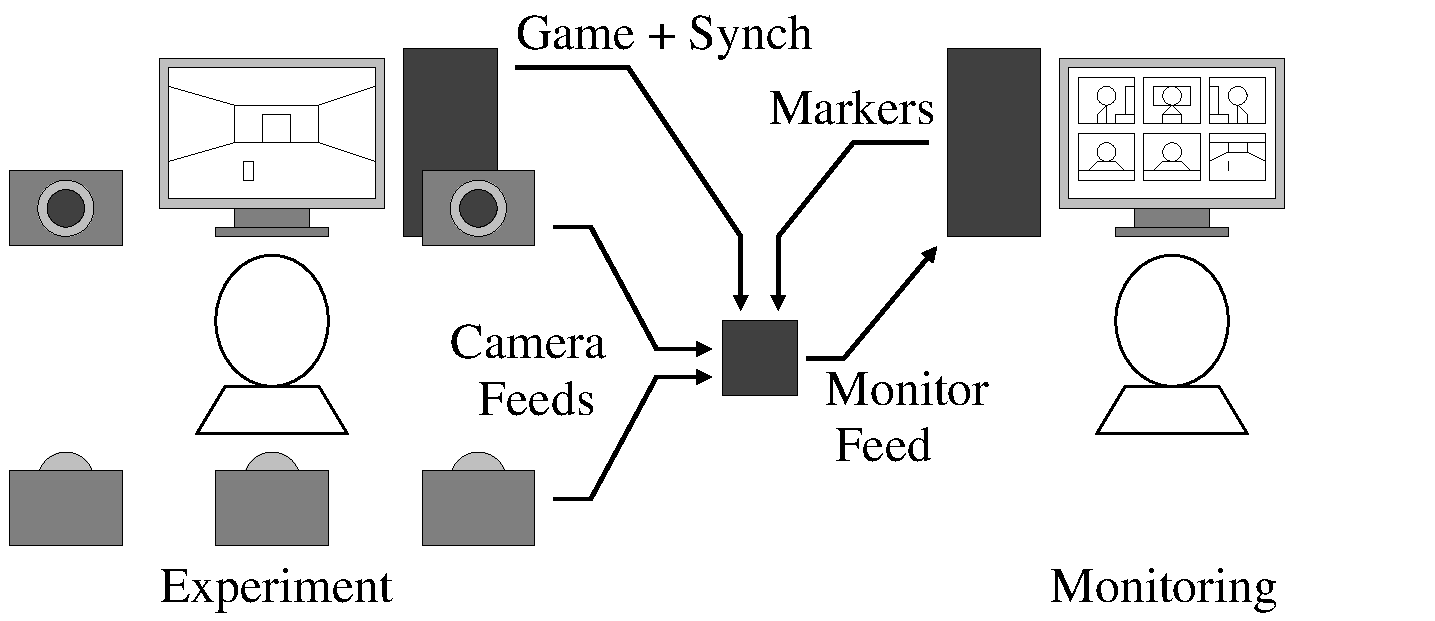
\includegraphics[width=0.95\textwidth]{figs/system-ext.pdf}
\end{center}
\caption{System block diagram.}\label{fig-system}
\end{figure}

The NeuroCam system processes several types of data and events (described
in detail in later sections):

\begin{itemize}

\item It collects frame data (with timestamps) from several cameras.

\item It collects streamed video data from the game machine.

\item It accepts web connections from authorized computers for control and
monitoring.

\item It provides a ``monitoring'' feed to the control computer showing
all video streams.

\item It records ``marker'' events when interface buttons are clicked on
the monitoring web page.

\item It records digital (TTL) signals from external equipment.

\item It accepts TTL ``start'' and ``stop'' signals from external equipment.

\item It offers collected data for examination, download, and
post-processing via a web interface after experiments have completed.

\end{itemize}

% NOTE - We can't mbox verbatim commands, so manually add line breaks.
To get started, connect an authorized machine to the ``\verb+neurocam+''
network and point it to \linebreak
``\verb+http://192.168.1.+\textit{(value)}''
(the IP address given on the sticker on the NeuroCam machine).

%
% This is the end of the file.

% NeuroCam manual - Hardware Setup
% Written by Christopher Thomas.
% Copyright (c) 2021 by Vanderbilt University. This work is released under
% the Creative Commons Attribution-ShareAlike 4.0 International License.

\chapter{Hardware Setup}
\label{setup}

The NeuroCam system has several hardware components:

\begin{itemize}

\item One ``NeuroCam'' embedded computer. This performs data collection and
storage.

\item One wireless router. This is connected to the NeuroCam computer and
to the game machine via wired LAN, and accepts wireless connections from
user machines. \textit{Do not connect this to the internet.}

The router used by the prototype system was an \mbox{Asus RT-N66U}.

\item One GPIO-and-synchronization box. This is connected to the NeuroCam
computer via USB, and provides TTL synchronization outputs over BNC and
accepts TTL-level inputs via a ribbon cable.

Any change in the TTL inputs is reported (and logged). A low-to-high
transition on bit 7 will start the NeuroCam recording, and a low-to-high
transition on bit 6 will stop recording (with a ``dead time'' of ten seconds
before further commands will be recognized). Input bits 0--5 are logged but
do not change NeuroCam behavior, and may be used for any desired purpose.

\item Five cameras, connected to the NeuroCam computer via USB.

The camera model used by the prototype system was the Logitech C920.

\end{itemize}

\begin{center}
% Black magic for the sizes here.
\begin{tabular}{cccc}
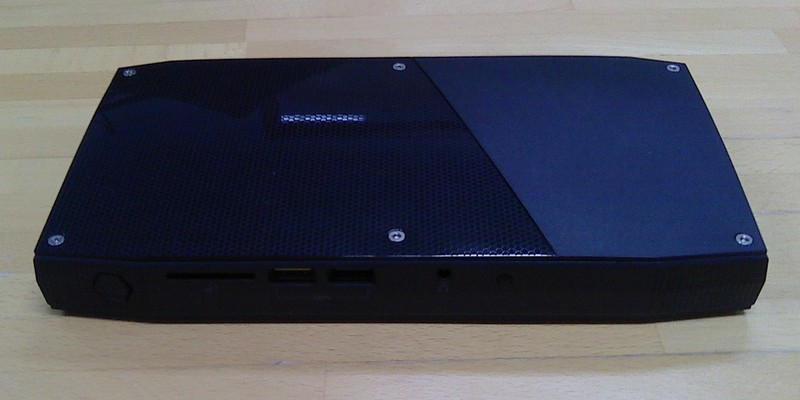
\includegraphics[height=0.14\textwidth]{pics-system/sys-comp-front.jpg} &
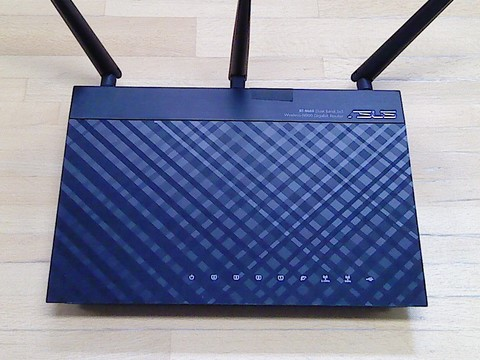
\includegraphics[height=0.14\textwidth]{pics-system/sys-router-front.jpg} &
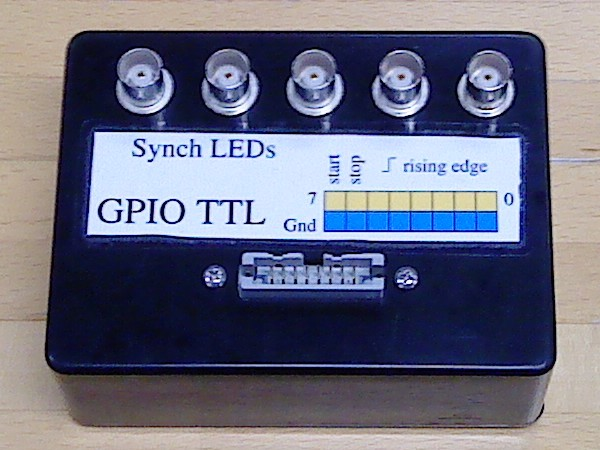
\includegraphics[height=0.14\textwidth]{pics-system/sys-gpio.jpg} &
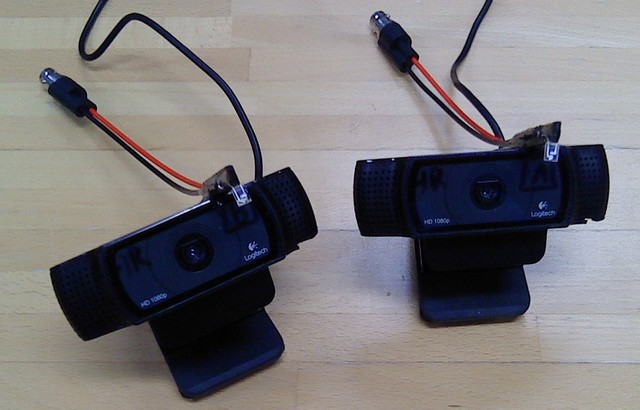
\includegraphics[height=0.14\textwidth]{pics-system/sys-cameras.jpg} \\
\end{tabular}
\end{center}

\clearpage

There are several tasks of note that have to be performed in order to
configure the NeuroCam hardware for use:

\begin{itemize}

\item The camera synchronization LEDs must be connected to the
GPIO-and-synchronization box via BNC cables.

Alternatively, a TTL-controlled lamp (visible or IR) may be placed in the
scene within view of all cameras and connected to the GPIO-and-synchronization
box.

\item The administrator password for the wireless router \textit{must} be
set to a new, stronger value. The default password (``administrator'') is
provided strictly for setup purposes.

The password for the NeuroCam network should also be changed. The default
password (``neurocam'') is easily guessed from the network name.

\item Any machines that are intended to communicate wirelessly with the
NeuroCam system must be added to the wireless router's MAC whitelist.
Machines that communicate via network cable may also need to be added,
depending on the router's configuration.

\item The game machine must be configured to stream MJPEG video, and to
respond to NeuroCam queries about offered content. The ``\verb+VLC+''
application was used for MJPEG streaming in the prototype system. Consult
VLC's documentation for further information.

Network handshaking with the game machine is described in Chapter 
\ref{handshake}.

\end{itemize}

The wireless router may be reconfigured by connecting to a wired LAN port
and accessing the web address printed on the bottom of the device.
\textbf{Do not} reset the device to factory default settings; this will lose 
all NeuroCam-related configuration.

See Chapter \ref{router} for details about configuring routers.

%
% This is the end of the file.

% NeuroCam manual - GUI
% Written by Christopher Thomas.
% Copyright (c) 2021 by Vanderbilt University. This work is released under
% the Creative Commons Attribution-ShareAlike 4.0 International License.

\chapter{Web Interface}
\label{gui}

The NeuroCam system has three interface screens: The \textbf{configuration}
screen, the \textbf{monitoring} screen, and the \textbf{repository browser}.
The monitoring screen is seen when the system is collecting data. When the
system is not collecting data, the configuration screen and the repository
browser are both available.

\textbf{Important:} Do not use the ``back'' button of your web browser to
switch pages. This will result in stale CGI information being submitted.
Use the navigation buttons in the NeuroCam application instead.

\section{Configuration Screen}
\label{gui-config}

\begin{figure}[h]
\begin{center}
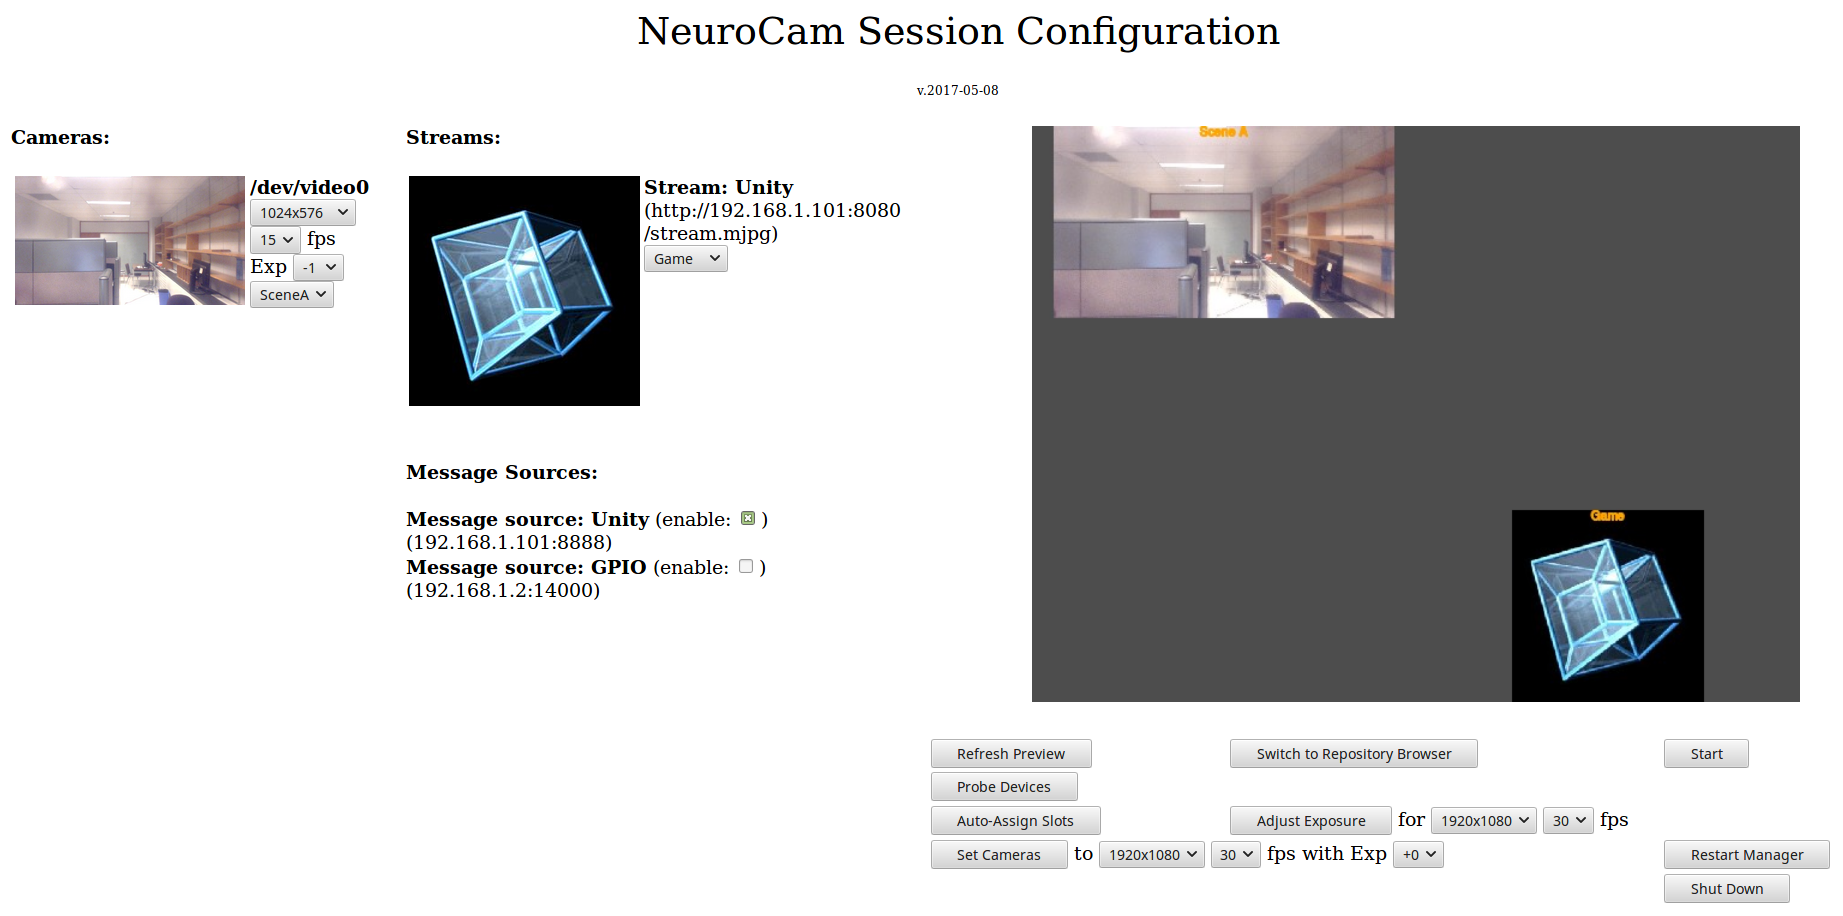
\includegraphics[width=0.95\textwidth]{pics-gui/gui-config.png}
\end{center}
\caption{Configuration screen.}\label{fig-gui-config}
\end{figure}

% FIXME - Annotate the image.

The configuration screen is used to set up a new video capture session.

Detected cameras are shown in the left column. The middle column shows
detected computer video streams and detected event message sources. The
right column shows a still-frame preview of the video feeds, with a control
panel under the preview.

Each camera has resolution, frame rate, and exposure settings, along with a
still-frame preview of its input. Longer (positive) exposures give a brighter
image but may reduce frame rate; shorter (negative) exposures give a dimmer
image but may increase frame rate. The ``slot'' to which the camera feed is
assigned may also be changed.

Camera settings may be changed all at once using the ``Set Cameras to...''
control in the control panel.

Camera settings may also be adjusted using the ``Adjust Exposure for...''
control in the control panel. This reduces exposure and resolution for each
camera until the specified frame rate is achieved. \textbf{Note:} this
adjustment takes several minutes (up to tens of minutes if the system has
difficulty finding appropriate settings).

There should always be at least one computer video stream, representing
a ``screencast'' of the game the subject is playing.

There should always be at least two event message sources: one from the game
computer (which sends game-time synchronization messages), and one from the
GPIO-and-synch box (which sends camera LED synchronization messages and
messages indicating changes in its TTL inputs).

The NeuroCam interface tries to enable appropriate message sources, choose
acceptable resolutions and frame rates, and assign appropriate feeds to
appropriate slots in the composite image, but some manual adjustment is
usually necessary. The ``Auto-Assign Slots'' control in the control panel
can be used to reset this assignment to the default.

The ``Refresh Preview'' button can be used to capture new images from the
cameras and computer video sources and to redraw the composite image preview.

\textbf{NOTE:} Some browsers may fail to update the preview images due to
cache behavior. Wait a moment and then click the ``preview'' button again
to refresh these images.

The ``Probe Devices'' button can be used to re-detect cameras, computer video
streams, and event/message feeds.

The ``Switch to Repository Browser'' button changes to the repository browser
screen, saving the configuration for later editing.

The ``Start'' button creates a new session directory, activates video capture,
and switches to the monitoring screen. This may alternatively be done by
raising the ``start capture'' TTL line.

The ``Restart Manager'' button forcibly restarts the NeuroCam software. This
allows recovery if any part of the NeuroCam software stops behaving correctly.
This is also needed if performing a software update without restarting the
NeuroCam machine.

The ``Shut Down'' button turns off the NeuroCam computer.

\section{Monitoring Screen}
\label{gui-monitor}

\begin{figure}[h]
\begin{center}
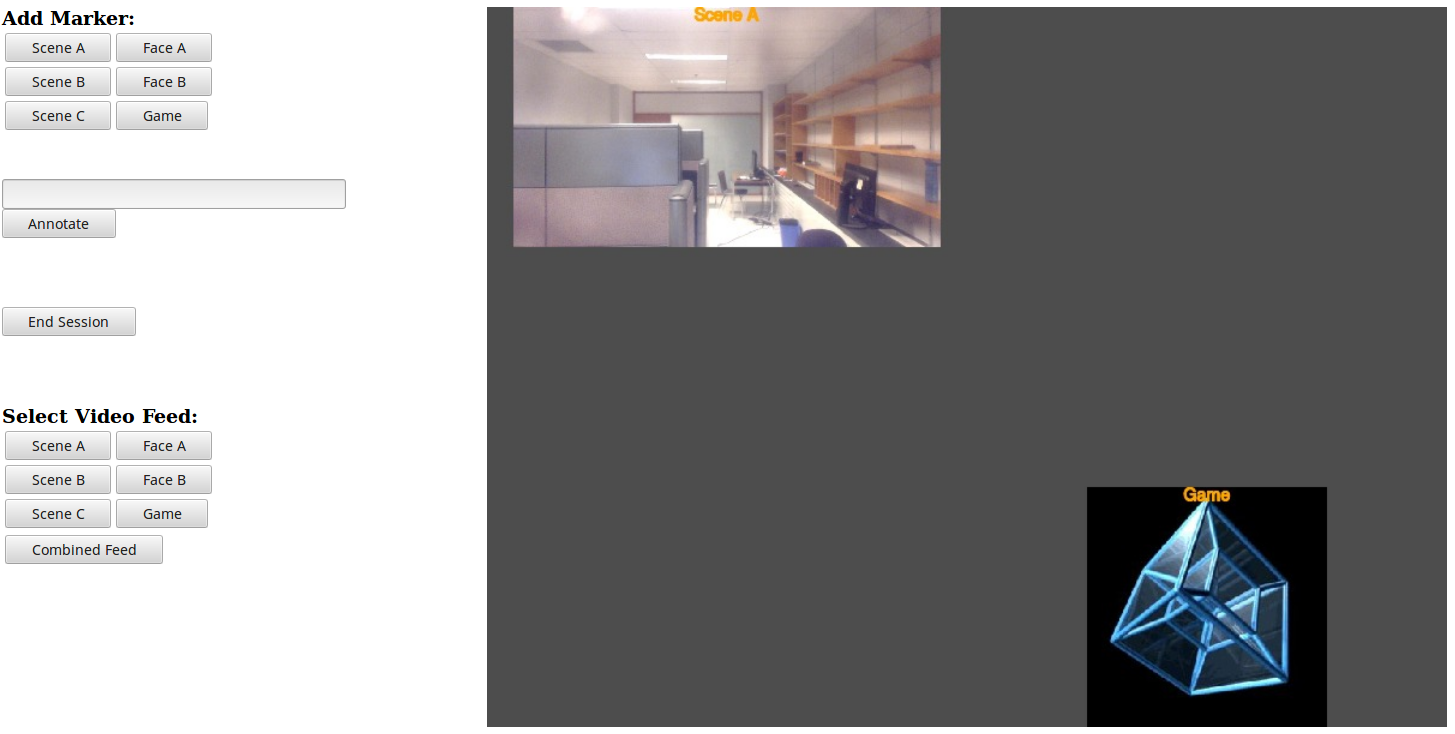
\includegraphics[width=0.95\textwidth]{pics-gui/gui-monitor.png}
\end{center}
\caption{Monitoring screen.}\label{fig-gui-monitor}
\end{figure}

% FIXME - Annotate the image.

The monitoring screen is used to view the progress of a capture session that
is underway, and to add event markers to the log file for this session.

The ``Add Marker'' buttons produce timestamped log entries indicating
events of interest in their respective video feeds.

The ``Annotate'' button produces a timestamped log entry containing
user-supplied text.

The ``End Session'' button stops video capture, closes the log file, and
switches to the repository browser screen. This may alternatively be done
by raising the ``stop capture'' TTL line.

The ``Select Video Feed'' buttons replace the combined image with the raw
video frames from the selected feed. This is usually better-quality and 
faster than the combined feed. The ``Combined Feed'' button returns to the
composite feed.

\section{Repository Browser}
\label{gui-repo}

\begin{figure}[h]
\begin{center}
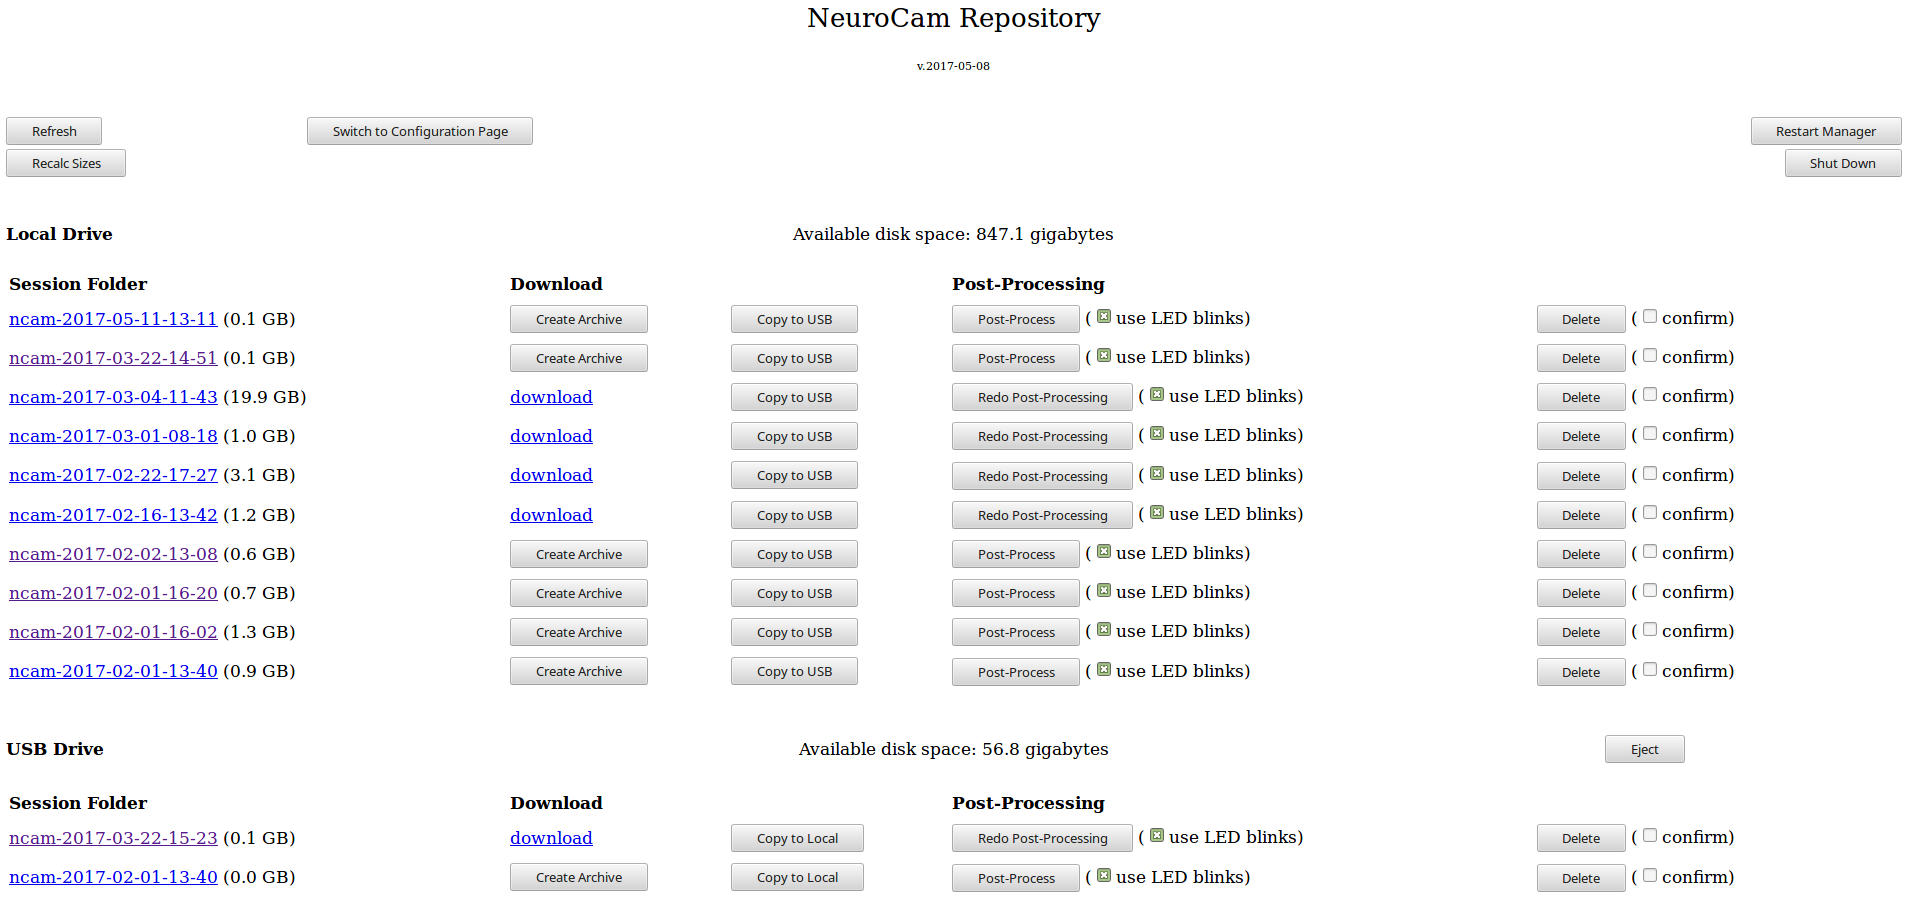
\includegraphics[width=0.95\textwidth]{pics-gui/gui-browser.png}
\end{center}
\caption{Repository browser.}\label{fig-gui-repo}
\end{figure}

% FIXME - Annotate the image.

The repository browser is used to inspect the data files produced by
past sessions, to perform post-processing of session data, and to download
and transfer packaged session data. Old sessions may also be deleted to free 
up disk space.

The ``Session Folder'' column lists sessions within the repository. Clicking
on a session name opens that session's directory in a new window. Files may
be individually inspected and downloaded via that window. See Chapter 
\ref{repo} for a description of the repository folder contents.

The ``Download'' column contains a link to a ``.tar'' archive containing
a session's entire directory tree. This is intended to provide an easy way
to transfer a session's data over the network. The archive is created using 
the ``Create Archive'' button. If post-processing has been performed, the 
archive includes the post-processed files. \textbf{NOTE:} The archive file 
is large. Check that there is sufficient free space before creating it.

The ``Copy to USB'' and ``Copy to Local'' buttons create duplicates of their
session folders on a USB-attached drive and on the local drive, respectively.
\textbf{NOTE:} These may instead be named ``Move to USB'' and ``Move to 
Local'', depending on settings. ``Move'' deletes the original folder, while
``Copy'' leaves it in place.

The ``Post-Processing'' button triggers several operations on a session 
folder. If the ``use LED blinks'' checkbox is set, video timestamps are
synchronized with each other using flashes of the infrared LEDs. A new log
file is saved with these adjusted timestamps. After synchronization, a
``Composite'' video feed is created, arranged in the same manner as the 
monitoring feed but at higher resolution and with full frame rate. A new log
file is saved with composite feed frame events added. Finally, movie files
of all video feeds are created for easy preview/playback.
\textbf{NOTE:} Post-processing operations take a lot of time on the local
drive (a solid-state drive), and even longer on magnetic platter or flash
drives.

\fixme{Benchmark post-processing. How long does processing an hour of
five-camera-plus-game footage take?}

The ``Delete'' buttons allow individual session folders (and their archives)
to be removed. This cannot be undone; to prevent accidental deletion, the
corresponding ``confirm'' checkbox must be checked before pressing the
``Delete'' button. Deleting old sessions will need to be performed frequently
in order to free up disk space.

The ``Eject'' button unmounts an external drive so that it can be safely
removed. \textbf{NOTE:} Writing data to an external drive can take a while,
so please wait until the NeuroCam indicates that it is safe for the drive
to be removed.

The ``Refresh'' button re-scans the repository directory for new sessions.

The ``Recalc Sizes'' button recomputes metadata for all session folders.
\textbf{NOTE:} This can take a while, as each session may contain millions
of files.

The ``Switch to Configuration Page'' button changes to the configuration
screen, so that the next capture session may be set up.

The ``Restart Manager'' button forcibly restarts the NeuroCam software. This
allows recovery if any part of the NeuroCam software stops behaving correctly.
This is also needed if performing a software update without restarting the
NeuroCam machine.

The ``Shut Down'' button turns off the NeuroCam computer.

%
% This is the end of the file.

% NeuroCam manual - Repository Data
% Written by Christopher Thomas.
% Copyright (c) 2021 by Vanderbilt University. This work is released under
% the Creative Commons Attribution-ShareAlike 4.0 International License.

\chapter{Repository Data}
\label{repo}

NeuroCam session data is stored in a ``repository''. Each session has its
own timestamped repository folder, containing some or all of the following:

\begin{itemize}

\item Raw video capture frames, stored as JPEG images in the ``Scene''
and ``Face'' folders.
\item Raw game capture frames, stored as JPEG images in the ``Game'' folder.

\item A ``Monitor'' folder containing reduced-size composited frames that
were sent to the monitoring GUI during the experiment. The composited frames
are not necessarily synchronized with each other.

\item A ``Composite'' folder containing larger composited frames produced
during post-processing. These composited frames should be synchronized.

\item A ``\verb+session.cfg+'' file containing information about the
settings used for the capture session. This file is described in detail in
Chapter \ref{structs}.

\item A ``\verb+logfile.txt+'' file containing raw event data (frame times,
user-supplied markers, and so forth).

\item Post-processed log files ``\verb+logfile-timed.txt+'' and
``\verb+logfile-composited.txt+''. The ``\verb+-timed+'' file has properly
synchronized timestamps and the ``\verb+-composited+'' file includes
timestamps for the ``Composite'' video stream (properly synchronized).

\item Several ``\verb+.mp4+'' compressed video files corresponding to the
video frame folders described above. These are lower-fidelity copies intended
to simplify review of footage.

\end{itemize}

% FIXME - Force a page break.
\clearpage
A typical session folder before post-processing is shown below:
\begin{center}
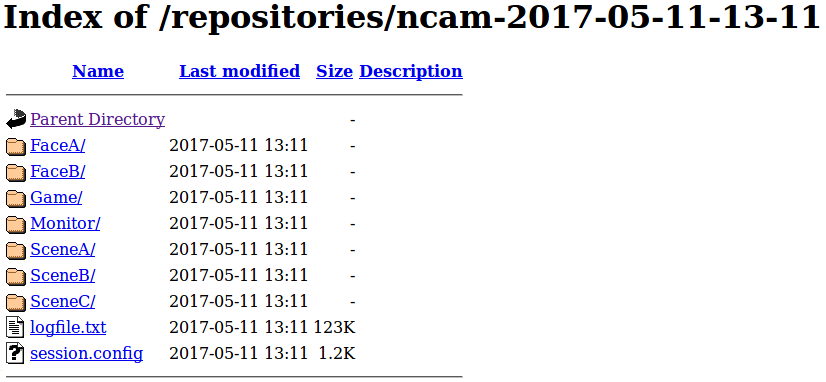
\includegraphics[width=0.6\textwidth]{pics-gui/gui-repo-unprocessed.png}
\end{center}

A typical session folder after post-processing is shown below:
\begin{center}
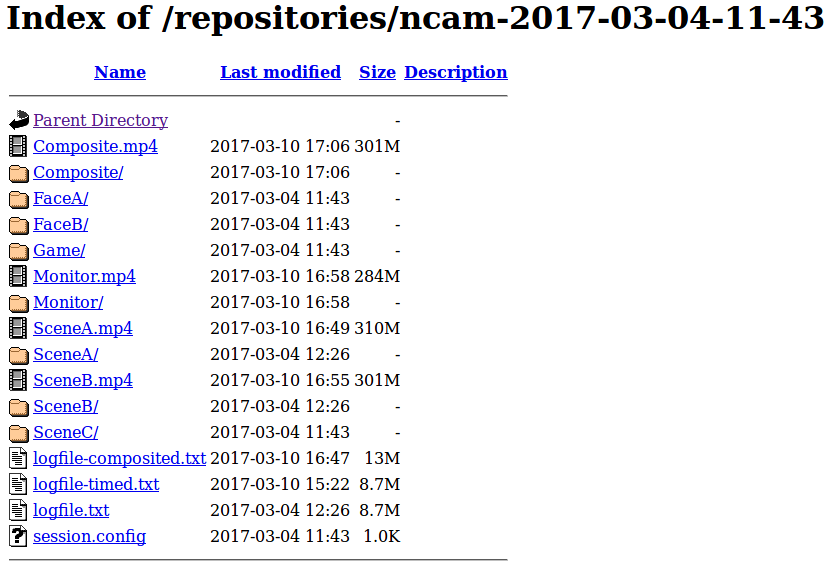
\includegraphics[width=0.6\textwidth]{pics-gui/gui-repo-afterprocess.png}
\end{center}

% FIXME - Force a page break.
\clearpage
\section{Log File Format}

The logfile is a human-readable text file recording one event per line. The 
following types of event are recorded:
\begin{itemize}
\item \textbf{Frame events}, indicating that a video frame was recorded.
This may be from a camera, from a remote computer video feed, or from a
generated feed like the ``Monitor'' and ``Composite'' feeds.
\item \textbf{Network message events}, which are typically sent by the
GPIO-and-synch box or by external applications such as the game.
\item \textbf{Local GUI events}, which are either user annotations, user
markers, or instructions to change the monitoring display.
\end{itemize}

\textbf{Frame events} indicate arrival time, stream ``slot'' name, sequence 
number, and the filename (including subfolder) where the frame was saved. 
Typical frame events are as follows:
\begin{verbatim}
(1367) [SceneA]  frame 8  SceneA/00000008.jpg
(1374) [SceneB]  frame 16  SceneB/00000016.jpg
(1382) [Monitor]  frame 36  Monitor/00000036.jpg
(1403) [SceneB]  frame 17  SceneB/00000017.jpg
(1417) [Monitor]  frame 37  Monitor/00000037.jpg
(1437) [SceneA]  frame 9  SceneA/00000009.jpg
(1444) [SceneB]  frame 18  SceneB/00000018.jpg
\end{verbatim}

\textbf{Netowrk events} indicate arrival time, IP and port of the source,
and a message string. Typical network events are as follows:
\begin{verbatim}
(304) [192.168.1.101:8888]  MSG Unity timestamp 53284 ms
(1303) [192.168.1.101:8888]  MSG Unity timestamp 54283 ms
(2303) [192.168.1.101:8888]  MSG Unity timestamp 55283 ms
(2795) [192.168.1.2:14000]  MSG gpio A0 O: 01
(2815) [192.168.1.2:14000]  MSG gpio A0 O: 00
(3303) [192.168.1.101:8888]  MSG Unity timestamp 56283 ms
(4303) [192.168.1.101:8888]  MSG Unity timestamp 57283 ms
\end{verbatim}

\textbf{Local GUI events} indicate event time, the fact that the event was
local, and a command, annotation, or marker string. Typical local events
are as follows:
\begin{verbatim}
(23197) [local]  CMD monitor SceneA
(39396) [local]  Marker: Game
(48249) [local]  CMD monitor Game
(76264) [local]  CMD monitor SceneA
(104119) [local]  CMD monitor Monitor
(491174) [local]  User annotation: "task started"
\end{verbatim}

%
% This is the end of the file.

% NeuroCam manual - Game Machine Handshaking
% Written by Christopher Thomas.
% Copyright (c) 2021 by Vanderbilt University. This work is released under
% the Creative Commons Attribution-ShareAlike 4.0 International License.

\chapter{Game Machine Handshaking}
\label{handshake}

The NeuroCam system queries machines on the local network to find content
providers. For the prototype system, the only network content provider is
the game machine.

The game machine should listen for UDP packets on port 8888. These will
be any of the following messages in plain text:
\begin{itemize}
\item ``\verb+looking for sources reply to port NNNN+''
\item ``\verb+talk to me on port NNNN+''
\item ``\verb+stop talking+''
\end{itemize}

The game machine may send any of the following responses:
\begin{itemize}
\item ``\verb+stream source at http://URL label XXXX+''
\item ``\verb+message source at HOST:PORT label XXXX+''
\item ``\verb+MSG (message text goes here)+''
\end{itemize}

The game machine will typically offer one video stream (the game video) and
one message source (which sends plain text timestamps for synchronization of
game events and NeuroCam data).

The video URL will generally be of the form
``\verb+http://(host IP):(port)/(file).mjpeg+''. Any valid URL should work,
as long as the file has the suffix ``\verb+mjpeg+'' and as long as the
host is given by IP address rather than hostname. This video stream will be
fetched by the NeuroCam and treated like any other camera feed.

Message sources must use IP addresses (not hostnames) as the host identifier.
These will be sent ``\verb+talk to me+'' and ``\verb+stop talking+''
messages, and when active are expected to send plain text UDP messages to
the NeuroCam machine. Messages are expected to begin with ``\verb+MSG +'',
with message content transcribed to the NeuroCam session log file. Message
source and NeuroCam timestamp information are also recorded in the log.

Multiple machines may respond to the broadcast query, and the same machine
may respond multiple times to one query. As long as the message and video
stream sources indicated by the responses are unique, they will all be
available to the NeuroCam system.

%
% This is the end of the file.


% FIXME - We need the router information too.
% This is normally in the maintenance section.
% NeuroCam manual - Router.
% Written by Christopher Thomas.
% Copyright (c) 2021 by Vanderbilt University. This work is released under
% the Creative Commons Attribution-ShareAlike 4.0 International License.

\chapter{Router}
\label{router}

The NeuroCam computer, the game machine, and user machines talk to each other
via a wireless router. Any modern router should be suitable.

All routers have different configuration interfaces, so consult the router's
manual for information on performing any given step.

The following configuration steps must be performed:
\begin{itemize}
%
\item \textbf{Reset to factory defaults if necessary.}

This can be done by holding down a small button on the rear or underside of
the router. \textbf{Do not do this after the router is configured} -- it will
undo all configuration, and it will all have to be done again.

\item \textbf{Update router firmware if necessary.}

This is done by downloading the new router firmware to a USB stick and
following the directions in the router's manual.

\item \textbf{Log into the router.}

This is done by connecting a notebook or desktop computer to one of the
router's LAN ports, and pointing a web browser to the IP address written on
the bottom of the router. This is usually ``\verb+http://192.168.1.1+''.

\item \textbf{Set the administrator password.}

The default login and password are written on a sticker on the router. These
are usually both set to ``\verb+admin+''. NeuroCam systems are configured to
use the login ``\verb+admin+'' and the password ``\verb+administrator+''.

\textbf{This is easily guessed, and so should be changed when the system is
installed per Chapter \ref{setup}.}

\item \textbf{Set the wireless SSID and password.}

The SSID is the name of the wireless network provided by the router. For
NeuroCam machines, this should have the form ``\verb+neurocam-NN+'', for
some unique number ``\verb+NN+''. Routers that offer 2.4~GHz and 5~GHz
networks separately should use the names ``\verb+neurocam-NN-2.4GHz+'' and
``\verb+neurocam-NN-5GHz+'' for those networks.

The wireless password should be set to ``\verb+neurocam+'' for new NeuroCam
systems. \textbf{This is easily guessed, and so should be changed when the
system is installed per Chapter \ref{setup}.}

\textbf{NOTE: Routers that offer 2.4~GHz and 5~GHz networks may need the
password to be set for each separately. Make sure both are set!}

\item \textbf{Enable and configure MAC address filtering.}

To provide additional security, the router should be configured to use
whitelist--based MAC address filtering (``default deny'' or ``default to
block'' policy). This will only allow machines to connect if their network
cards belong to a list supplied during router configuration.

The MAC address of the machine being used to configure the router should be
added to the list before enabling filtering. If known, the MAC addresses for
other user machines may be added as well.

The MAC address of the NeuroCam machine and of the game machine will often
also have to be added. This depends on exactly how the router implements
filtering (some filter inbound wireless connections, others filter both
wireless and LAN connections). When in doubt, add the NeuroCam and game
machines to the whitelist.

To find the MAC address of a Linux machine, type ``\verb+ifconfig+''
(or ``\verb+/sbin/ifconfig+'') at a command prompt and look for the
``\verb+HWaddr+'' field.

\textbf{NOTE: Routers that offer 2.4~GHz and 5~GHz networks need MAC address
filtering set up separately, and saved, for each. Make sure it's set up for
both!}

\item \textbf{Add static IP assignments.}

The router normally dynamically assigns IP addresses to clients (including
the NeuroCam machine and the game machine).

Known machines can be assigned fixed IP addresses. At minimum the NeuroCam
machine should be given a fixed IP address. These usually take the form
``\verb+192.168.1.NN+'', where NN is the number of the NeuroCam computer.

\textbf{NOTE:} Some routers use a number other than ``\verb+1+'' in
``\verb+192.168.1.NN+''. Where possible, the DHCP configuration should be
changed to make this ``\verb+1+'', for consistency between installations.

\textbf{NOTE:} The router may have a ``device name''. This should be set
to ``\verb+neurocam-NN-gw+'' (where ``\verb+NN+'' is the same number from
the SSID, described above). The ``\verb+-gw+'' suffix guarantees that this
will not conflict with any NeuroCam computer name.

\item \textbf{Cover the WAN port (internet port).}

The NeuroCam system should never be connected to the internet, as it is not
hardened against attack. To avoid confusion between the WAN (internet) port
and the LAN (local network) ports, place a sticker or piece of tape over the
WAN port.
%
\end{itemize}

The preferred router for the NeuroCam prototype was as follows:

\begin{tabular}{llll}\hline
Qty & Description & Manuf. p/n & NewEgg SKU \\
\hline
%
1 & wireless router (a/b/g/n) & Asus RT-N66U & N82E16833320091 \\
%
\hline
\end{tabular}

%
%
\clearpage
\section{Asus RT-N66U Screenshots}

This is the Asus RT-N66U router (with tape over the WAN port):
\begin{center}
\begin{tabular}{ccc}
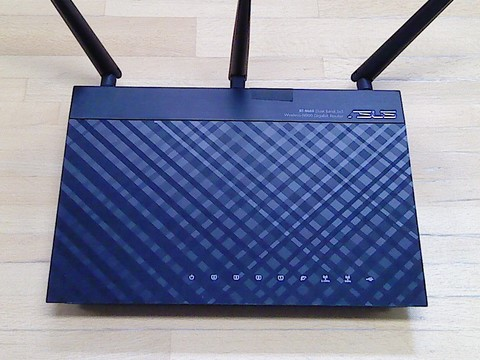
\includegraphics[width=0.35\textwidth]{pics-system/sys-router-front.jpg} &
~ &
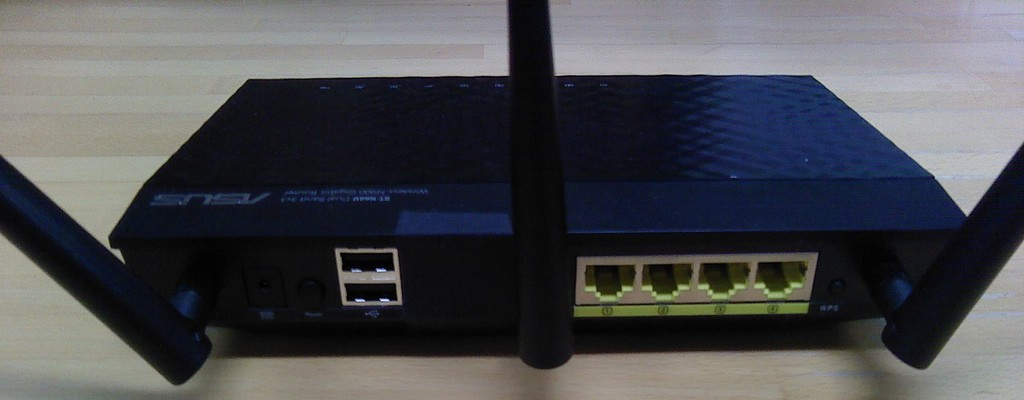
\includegraphics[width=0.45\textwidth]{pics-system/sys-router-back.jpg} \\
\end{tabular}
\end{center}

Changing the administrator login/password (top section):
\begin{center}
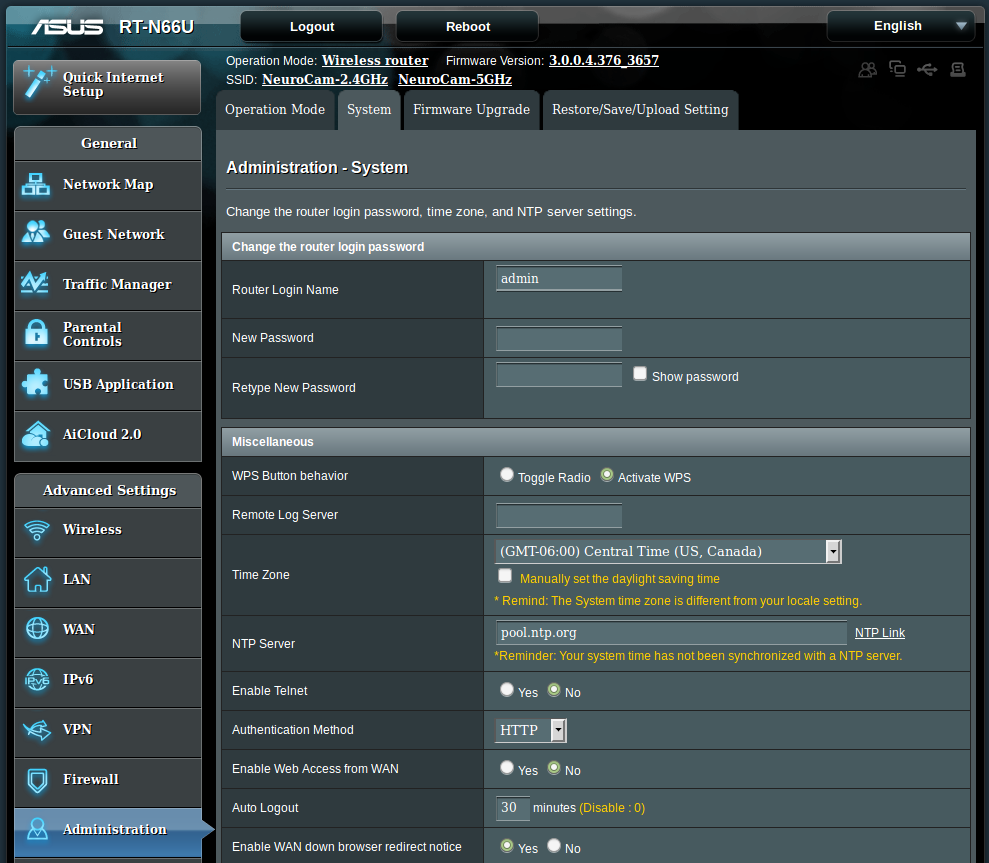
\includegraphics[width=0.7\textwidth]
{pics-router/asus-n66u-admin-pw.png}
\end{center}

% Force a page break.
\clearpage
Setting the wireless network name (``SSID'') and password (``pre-shared 
key''):
\begin{center}
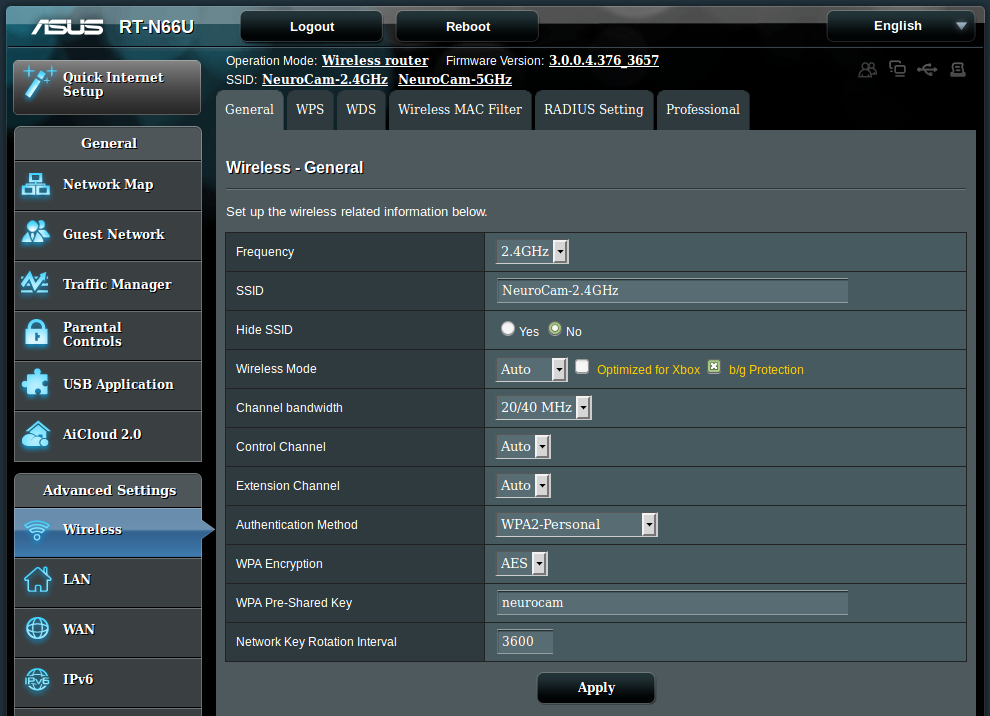
\includegraphics[width=0.7\textwidth]
{pics-router/asus-n66u-ssid.png}
\end{center}

Changing the MAC filter to whitelist mode (``accept the specified 
addresses''), and adding addresses:
\begin{center}
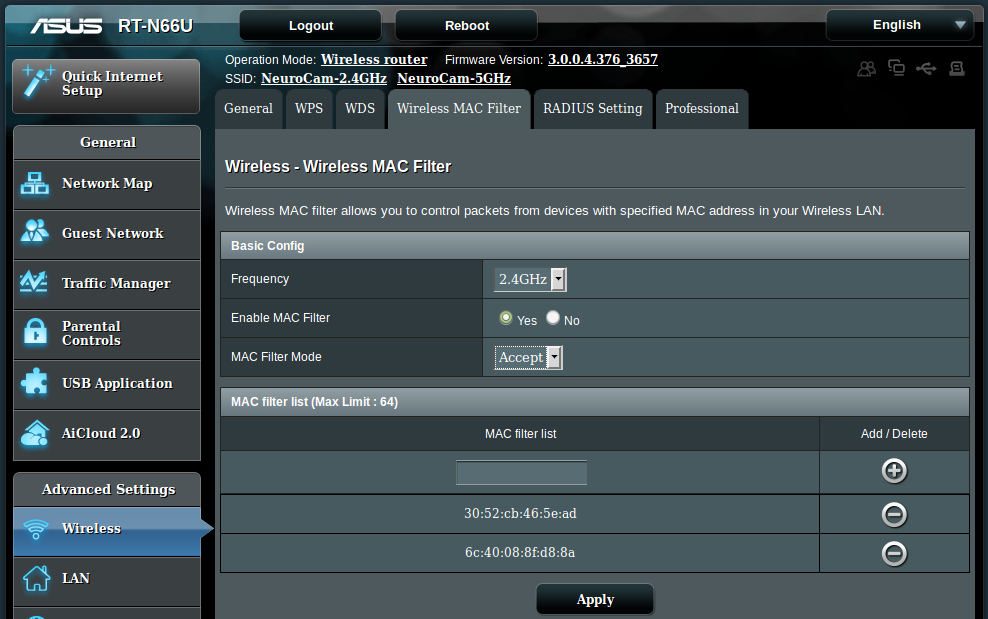
\includegraphics[width=0.7\textwidth]
{pics-router/asus-n66u-macfilter.png}
\end{center}

% Force a page break.
\clearpage
Assigning static IP addresses to specific machines:
\begin{center}
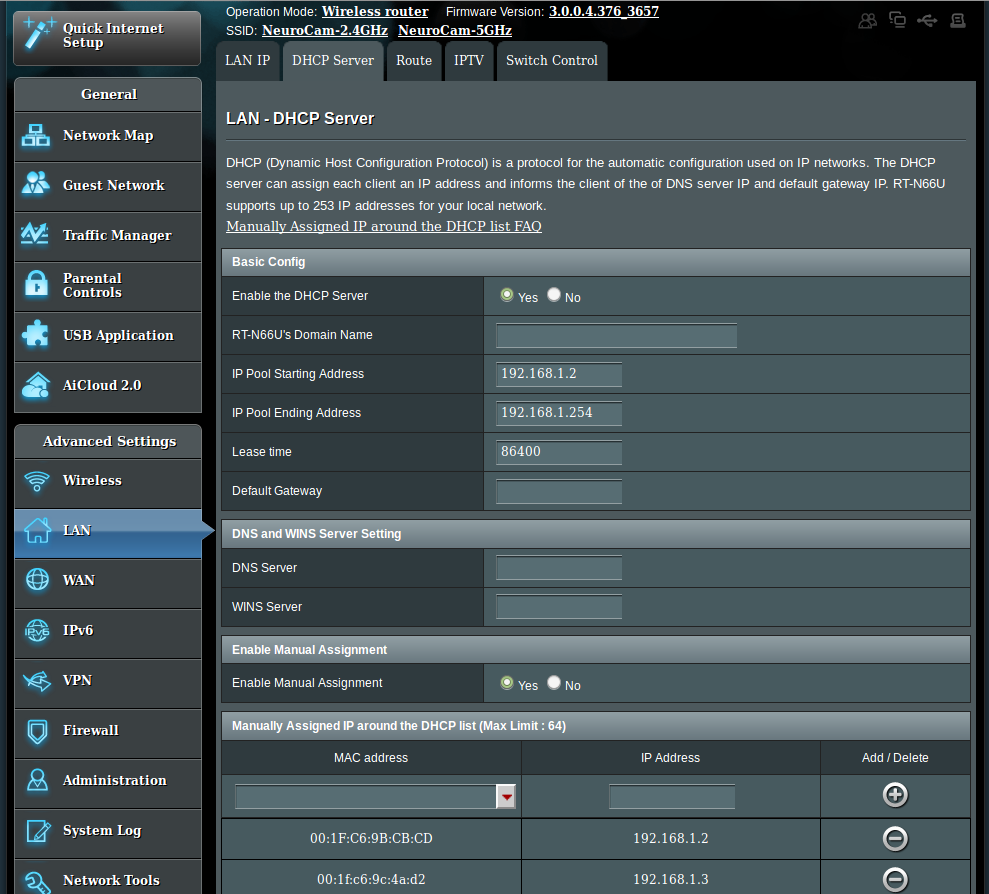
\includegraphics[width=0.7\textwidth]
{pics-router/asus-n66u-static.png}
\end{center}

%
%
\clearpage
\section{Installing OpenWrt}

\fixme{This hasn't been implemented, so no documentation for it.}

{\itshape The idea is to provide scripts that automatically configure and
compile the ``\verb+OpenWrt+'' open--source firmware. This lets us lock down
any features we don't want active, force an appropriate filtering mode, and
disable the web interface (which is one of the main security holes).

Implementing this is deferred, as it will be time--consuming.}

%
% This is the end of the file.


\end{document}

%
% This is the end of the file.
